\eventsection{RESULTADOS E DISCUSS\~AO}

Os resultados obtidos indicam que o sistema \'e capaz de apoiar o monitoramento ambiental do Lago do Serpa com respostas num\'ericas consistentes para os par\^ametros analisados. No melhor arranjo avaliado, os erros absolutos m\'edios foram de 0,107 para pH, 0,222 para oxig\^enio dissolvido e 0,971 para turbidez. Em termos pr\'aticos, esses valores mostram que a solu\c{c}\~ao pode apoiar leituras de campo com boa estabilidade para pH e oxig\^enio dissolvido, enquanto a turbidez exige interpreta\c{c}\~ao mais cautelosa, mas ainda \'e \'util para triagem ambiental e defini\c{c}\~ao de novas coletas.

Essa diferen\c{c}a de comportamento tem implica\c{c}\~ao direta para o uso da ferramenta. Em situa\c{c}\~oes de monitoramento ambiental, resultados mais est\'aveis para pH e oxig\^enio dissolvido oferecem suporte importante para acompanhamento das condi\c{c}\~oes da \'agua e para a comunica\c{c}\~ao com equipes locais. No caso da turbidez, embora a incerteza seja maior, a resposta do sistema permanece \'util como indicador de alerta e como apoio \`a tomada de decis\~ao em regi\~oes remotas.

\begin{table}[H]
\centering
\caption{Indicadores de desempenho do sistema para os par\^ametros monitorados.}
\label{tab:desempenho}
\tabelafonte
\begin{tabular}{lc}
\toprule
Par\^ametro & Erro absoluto m\'edio \\
\midrule
pH & 0,107 \\
Oxig\^enio dissolvido & 0,222 \\
Turbidez & 0,971 \\
\bottomrule
\end{tabular}
\artigofonte{elabora\c{c}\~ao pr\'opria com base nos experimentos do estudo de base.}
\end{table}

Tomado isoladamente, esse resultado pontual n\~ao responde se o erro obtido \'e efetivamente competitivo. Por essa raz\~ao, o estudo de base tamb\'em comparou o modelo proposto com tr\^es baselines consolidados: Random Forest, LSTM e MLP. A Tabela \ref{tab:baselines} mostra que, em erro macro m\'edio, Random Forest e LSTM apresentaram desempenho preditivo superior no mesmo conjunto de dados, enquanto o MLP exibiu pior comportamento e forte instabilidade. Assim, a leitura correta n\~ao \'e a de superioridade universal da rede espiculada, mas a de uma solu\c{c}\~ao que preserva desempenho competitivo ao mesmo tempo em que viabiliza processamento local em hardware restrito.

\begin{table}[H]
\centering
\caption{Comparativo multissemente entre o modelo proposto e baselines cl\'assicos.}
\label{tab:baselines}
\tabelafonte
\begin{tabular}{lccc}
\toprule
Modelo & MAE macro & RMSE macro & $R^2$ macro \\
\midrule
Random Forest & 0,409 $\pm$ 0,062 & 0,557 $\pm$ 0,086 & 0,335 $\pm$ 0,131 \\
LSTM & 0,428 $\pm$ 0,059 & 0,548 $\pm$ 0,073 & 0,313 $\pm$ 0,139 \\
SNN multimodal & 0,447 $\pm$ 0,064 & 0,566 $\pm$ 0,072 & 0,291 $\pm$ 0,146 \\
MLP & 0,781 $\pm$ 0,193 & 0,983 $\pm$ 0,178 & -5,460 $\pm$ 5,220 \\
\bottomrule
\end{tabular}
\artigofonte{elabora\c{c}\~ao pr\'opria com base no benchmark multissemente do estudo de base.}
\end{table}

Essa compara\c{c}\~ao \'e decisiva para interpretar a escolha do modelo. Do ponto de vista estritamente preditivo, a arquitetura espiculada n\~ao superou os melhores baselines nesta base local. Sua justificativa t\'ecnica est\'a na combina\c{c}\~ao entre erro aceit\'avel, infer\^encia offline, compatibilidade com exporta\c{c}\~ao para TFLite e potencial de execu\c{c}\~ao em dispositivos de borda como Android, Raspberry Pi e ESP32. Em cen\'arios remotos, esse compromisso entre desempenho e implantabilidade pode ser mais relevante do que a melhor m\'etrica isolada.

Outro aspecto que merece destaque \'e a robustez. O benchmark com dez sementes independentes mostrou que o SNN apresentou MAE macro de 0,447 $\pm$ 0,064, RMSE macro de 0,566 $\pm$ 0,072 e $R^2$ macro de 0,291 $\pm$ 0,146. Esses desvios-padr\~ao n\~ao eliminam a variabilidade esperada de uma base pequena, mas mostram que o comportamento do modelo n\~ao depende de uma \'unica divis\~ao fortuita dos dados. Em contraste, o MLP apresentou dispers\~ao muito maior, o que refor\c{c}a a import\^ancia de discutir estabilidade experimental e n\~ao apenas o melhor MAE encontrado.

Do ponto de vista estat\'istico, tamb\'em cabe cautela. No teste de sinal pareado entre SNN e Random Forest, n\~ao houve evid\^encia de superioridade global do SNN nas m\'etricas macro ao n\'ivel de 5\% de signific\^ancia. Esse resultado refor\c{c}a que a proposta deve ser defendida principalmente por sua viabilidade operacional e territorial, e n\~ao por uma suposta lideran\c{c}a absoluta em acur\'acia dentro desta base.

A interpreta\c{c}\~ao pr\'atica dos resultados se torna mais clara quando as estimativas s\~ao observadas espacialmente. Em vez de focar apenas na compara\c{c}\~ao entre valores previstos e observados, esta vers\~ao do artigo enfatiza a leitura territorial das condi\c{c}\~oes do lago. Isso torna a discuss\~ao mais compat\'ivel com aplica\c{c}\~oes de monitoramento ambiental.

\begin{figure}[H]
\centering
\caption{Painel espacial reconfigurado dos par\^ametros monitorados no Lago do Serpa. Nos mapas, $x$ representa a coordenada leste e $y$ a coordenada norte no sistema UTM 21S, em metros.}
\label{fig:idw_individual}
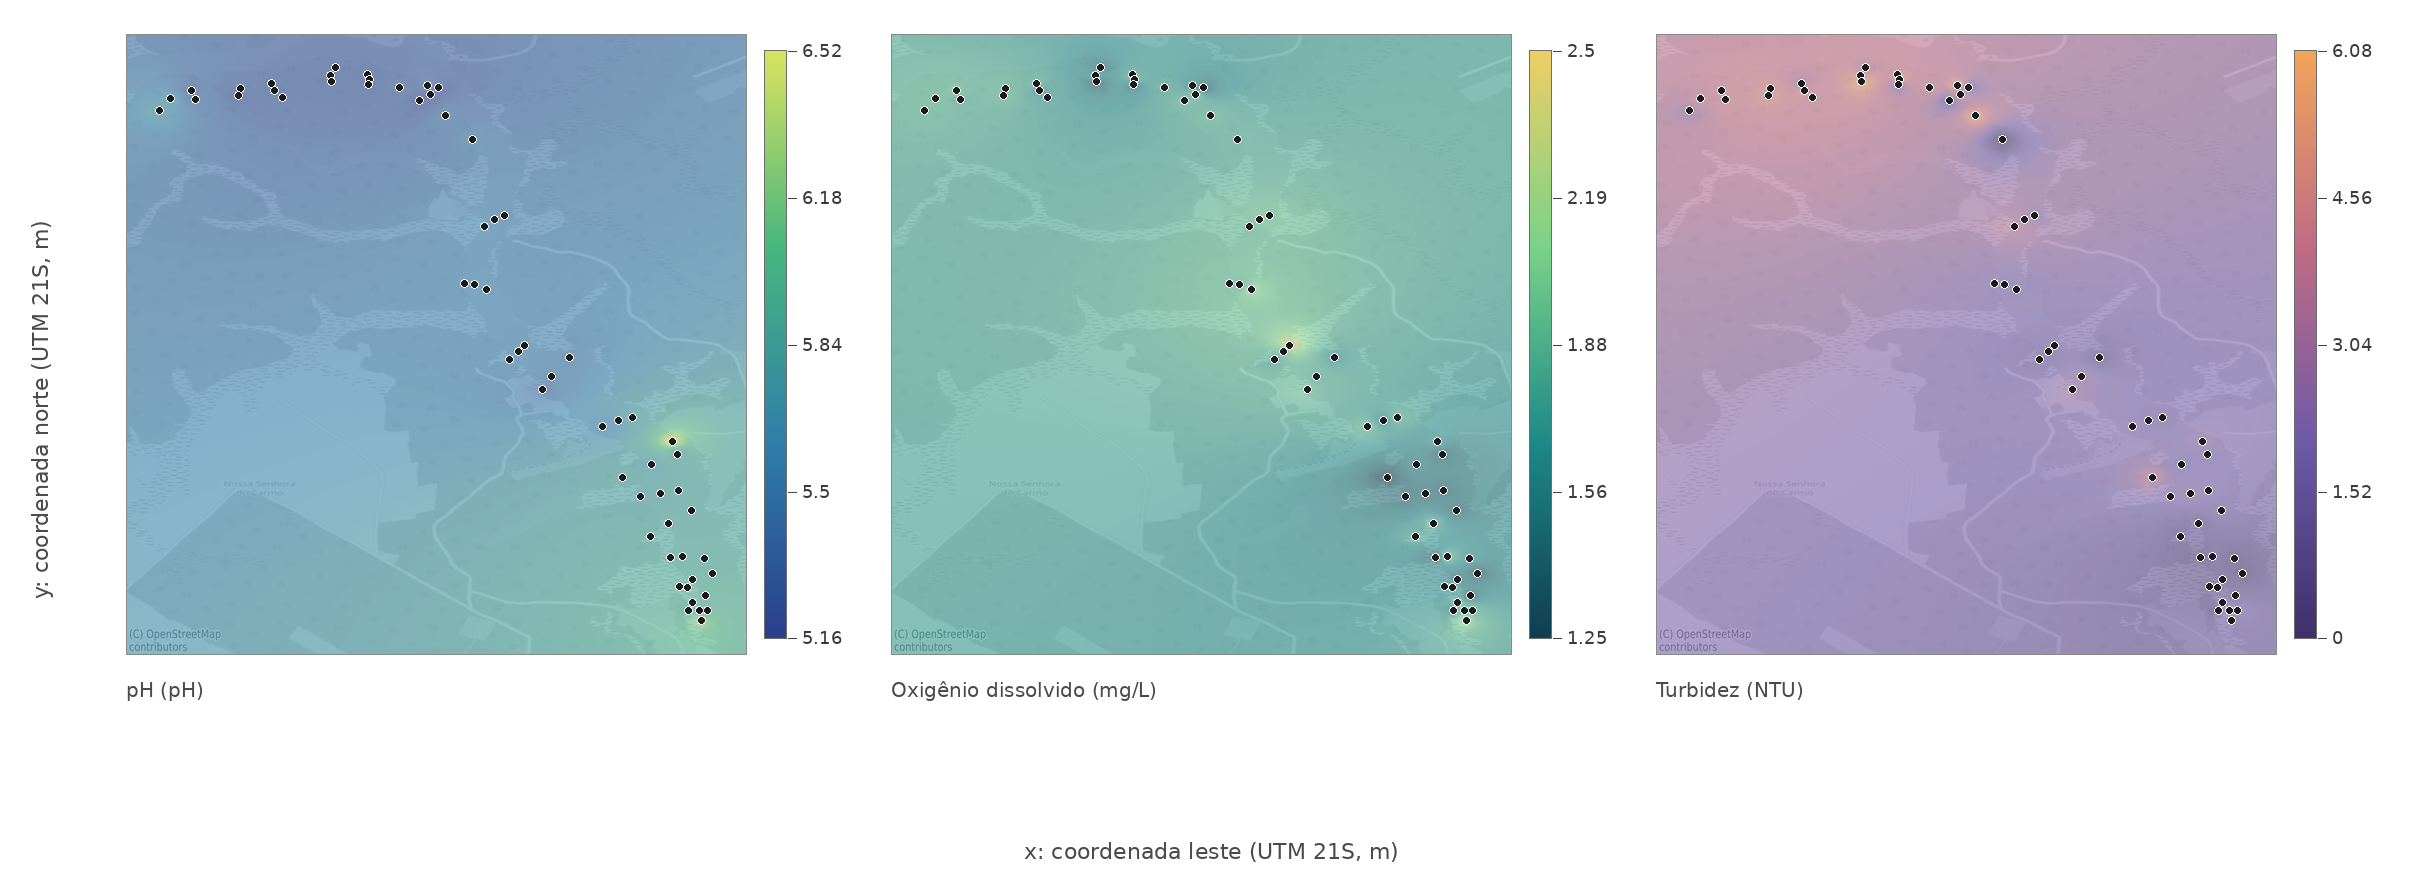
\includegraphics[width=0.98\textwidth]{idw_triptych_redesigned.png}
\artigofonte{elabora\c{c}\~ao pr\'opria com base nas superf\'icies interpoladas do estudo.}
\end{figure}

A Figura \ref{fig:idw_individual} evidencia que a proposta n\~ao se resume \`a gera\c{c}\~ao de valores num\'ericos. Ao produzir uma leitura espacialmente organizada, o sistema contribui para o planejamento de novas coletas, para a comunica\c{c}\~ao dos resultados e para a prioriza\c{c}\~ao de trechos com maior interesse ambiental. Esse tipo de leitura pode ser particularmente relevante para comunidades ribeirinhas e equipes de campo com acesso limitado a laborat\'orios e internet. No que se refere \`a implanta\c{c}\~ao em hardware, a proposta tamb\'em se mostrou vi\'avel. Na Raspberry Pi 4B, a lat\^encia m\'edia foi de 0,214 ms por amostra, com vaz\~ao de 4670,50 amostras por segundo. Em dispositivos Android, os valores foram mais elevados, com destaque para o Device B, que alcan\c{c}ou 30905,08 amostras por segundo. No ESP32, a taxa de 5,0 amostras por segundo indica uma opera\c{c}\~ao mais simples, mas ainda compat\'ivel com monitoramento peri\'odico e aut\^onomo em cen\'arios de baixa conectividade.

\begin{table}[H]
\centering
\caption{Viabilidade operacional do sistema em diferentes plataformas de borda.}
\label{tab:plataformas}
\tabelafonte
\begin{tabular}{lc}
\toprule
Plataforma & Vaz\~ao (amostras/s) \\
\midrule
ESP32 & 5,0 \\
Raspberry Pi 4B & 4670,50 \\
Android A & 12337,40 \\
Android B & 30905,08 \\
Android C & 16121,71 \\
\bottomrule
\end{tabular}
\artigofonte{elabora\c{c}\~ao pr\'opria a partir dos ensaios de execu\c{c}\~ao do sistema.}
\end{table}

Os resultados de execu\c{c}\~ao ajudam, portanto, a distinguir cen\'arios de uso. O ESP32 pode atender a rotinas mais simples e esparsas de monitoramento, o que favorece aplica\c{c}\~oes peri\'odicas e aut\^onomas. J\'a Android e Raspberry Pi oferecem condi\c{c}\~oes mais favor\'aveis quando h\'a necessidade de maior frequ\^encia de processamento, visualiza\c{c}\~ao local, intera\c{c}\~ao com usu\'arios e apoio mais imediato \`a tomada de decis\~ao.

Sob a perspectiva de utilidade social, a leitura espacial dos par\^ametros j\'a oferece valor concreto. Em vez de limitar a interpreta\c{c}\~ao a tabelas t\'ecnicas, o sistema permite uma vis\~ao mais imediata de onde a aten\c{c}\~ao deve ser concentrada. Com isso, o di\'alogo com gestores, equipes de campo, servi\c{c}os de vigil\^ancia ambiental e comunidades locais tende a se tornar mais direto, ampliando o potencial de uso da proposta para al\'em do ambiente estritamente acad\^emico. Outro aspecto relevante \'e a possibilidade de uso progressivo da solu\c{c}\~ao. Em um primeiro momento, o sistema pode funcionar como instrumento complementar de triagem, auxiliando equipes em coletas explorat\'orias e em campanhas pontuais. Em uma etapa posterior, com amplia\c{c}\~ao do conjunto de dados e adapta\c{c}\~ao a outros ambientes aqu\'aticos, a mesma estrutura pode apoiar rotinas mais frequentes de monitoramento territorial.

Esse potencial de expans\~ao \'e importante porque mostra que a proposta n\~ao est\'a restrita a um experimento isolado. Ao contr\'ario, trata-se de uma base tecnol\'ogica que pode ser incrementada em novas campanhas, integrada a outras vari\'aveis ambientais e ajustada a diferentes realidades amaz\^onicas. Mesmo mantendo car\'ater aplicado e de baixo custo, o sistema apresenta perspectiva de continuidade e replicabilidade. Do ponto de vista aplicado, os achados mostram que o sistema pode ser inserido em rotinas de monitoramento em regi\~oes remotas, nas quais a continuidade do acompanhamento depende de solu\c{c}\~oes aut\^onomas, simples e de menor custo. O funcionamento offline amplia o potencial de uso em comunidades ribeirinhas, campanhas de vigil\^ancia ambiental e a\c{c}\~oes de apoio \`a sa\'ude p\'ublica. Ao mesmo tempo, essa interpreta\c{c}\~ao ainda n\~ao equivale a valida\c{c}\~ao externa: como toda a an\'alise foi conduzida com dados do Lago do Serpa, permanece em aberto o desempenho da solu\c{c}\~ao em outros lagos ou contextos amaz\^onicos.

Al\'em disso, o estudo refor\c{c}a um ponto central: o diferencial do artigo n\~ao est\'a em disputar originalidade apenas pelo desenho t\'ecnico do modelo, mas em demonstrar uma aplica\c{c}\~ao concreta e territorialmente situada. Em contextos marcados por baixa conectividade, longas dist\^ancias e forte depend\^encia dos recursos h\'idricos, uma solu\c{c}\~ao embarcada e funcional pode gerar impacto pr\'atico superior ao de abordagens voltadas exclusivamente \`a compara\c{c}\~ao t\'ecnica.

Em s\'intese, os resultados sustentam uma interpreta\c{c}\~ao em duas frentes complementares. A primeira \'e ambiental, ao mostrar que o sistema consegue estimar vari\'aveis relevantes da qualidade da \'agua. A segunda \'e operacional, ao indicar que essa capacidade pode ser levada para dispositivos de campo e convertida em apoio concreto ao monitoramento ambiental, \`a sa\'ude p\'ublica e \`a tomada de decis\~ao na Amaz\^onia.

\eventsubsection{Implica\c{c}\~oes para uso em campo}

Quando se considera o uso do sistema fora do ambiente acad\^emico, alguns pontos ganham destaque. O primeiro deles \'e a possibilidade de reduzir a depend\^encia de processamento remoto em cen\'arios onde a internet \'e limitada. Em muitos territ\'orios amaz\^onicos, a dificuldade n\~ao est\'a apenas em coletar a informa\c{c}\~ao, mas em conseguir transform\'a-la rapidamente em uma leitura \'util para a equipe que est\'a no local. Ao operar no pr\'oprio dispositivo, a solu\c{c}\~ao encurta esse caminho. O segundo ponto est\'a relacionado ao car\'ater progressivo do monitoramento. Em vez de substituir procedimentos tradicionais, o sistema pode atuar como ferramenta complementar, ajudando a indicar onde novas coletas devem ser priorizadas e quais trechos do lago merecem aten\c{c}\~ao mais imediata. Esse tipo de apoio \'e especialmente relevante quando os recursos humanos e log\'isticos s\~ao limitados.

Tamb\'em \'e importante observar que a aplica\c{c}\~ao em campo envolve diferentes perfis de usu\'ario. Pesquisadores, gestores locais, t\'ecnicos ambientais e equipes de apoio podem se beneficiar de uma sa\'ida mais objetiva, baseada em mapas, indicadores e previs\~oes acess\'iveis. Isso amplia a utilidade da proposta, pois a transforma em um recurso de comunica\c{c}\~ao e triagem, n\~ao se tratando, portanto, apenas de uma experi\^encia computacional. Por fim, a experi\^encia com o Lago do Serpa sugere que abordagens desse tipo podem fortalecer estrat\'egias de monitoramento territorial na Amaz\^onia. Mesmo com limita\c{c}\~oes de base de dados, a solu\c{c}\~ao demonstrou que \'e poss\'ivel integrar medi\c{c}\~oes locais, processamento embarcado e leitura espacial em uma estrutura tecnol\'ogica coerente com as condi\c{c}\~oes de regi\~oes remotas, embora a generaliza\c{c}\~ao para outros corpos h\'idricos ainda dependa de valida\c{c}\~ao adicional.
